\documentclass{TDP003mall}
\usepackage{listings}
\usepackage{color}
\usepackage{listings}
\usepackage{hyperref}
\usepackage{graphicx}
\definecolor{grey}{gray}{0.9}


\lstset{%
language=Lisp,
basicstyle=\small,
backgroundcolor=\color{grey},
mathescape=true}

\newcommand{\version}{Version 0.5}
\author{Jessk378, Nikni292}
\title{systemdokumentation}
\date{2015-10-06}
\rhead{jessk378, Nikni292}



\begin{document}
\projectpage
\section{Revisionshistorik}
\begin{table}[!h]
\begin{tabularx}{\linewidth}{|l|X|l|}\hline
Ver. & Revisionsbeskrivning & Datum \\\hline
0.1 & skapade dokument för skrivning & 151006\\\hline
0.2 & La in sekvensdiagram och översikts bild & 151008\\\hline
1.0 & Färdigställde information om presentationslagret & 151008\\\hline
\end{tabularx}
\end{table}
\pagebreak
\tableofcontents
\newpage

\section{Introduktion}
I detta dokument kommer ni ta del av hur våran kod är tänkt att fugera. Ni kommer se sekvensdiagram över hur våra funktioner fungerar med varandra, samt bilder med förklaringar på specifika kodstycken.

\section{Sekvensdiagram}
Användaren står på söksidan och gör en sökning. Sök strängen skickas till flask som då kallar på sök funktionen i datalagret. Den utförs i tre steg, först hittas alla projekt som innehåller strängen, den kollar sedan om det finns angivna tekniker om det finns filtrerar den ut alla projekt som inte har med teknikerna, det sista sök funktionen gör är att sortera datat utifrån vad som angetts. Den skickar sedan tillbaka den sökta datan till flask som kallar på jinja att ladda in resultat i sök hmtl sidan.
\begin{figure}[ht!]
\centering
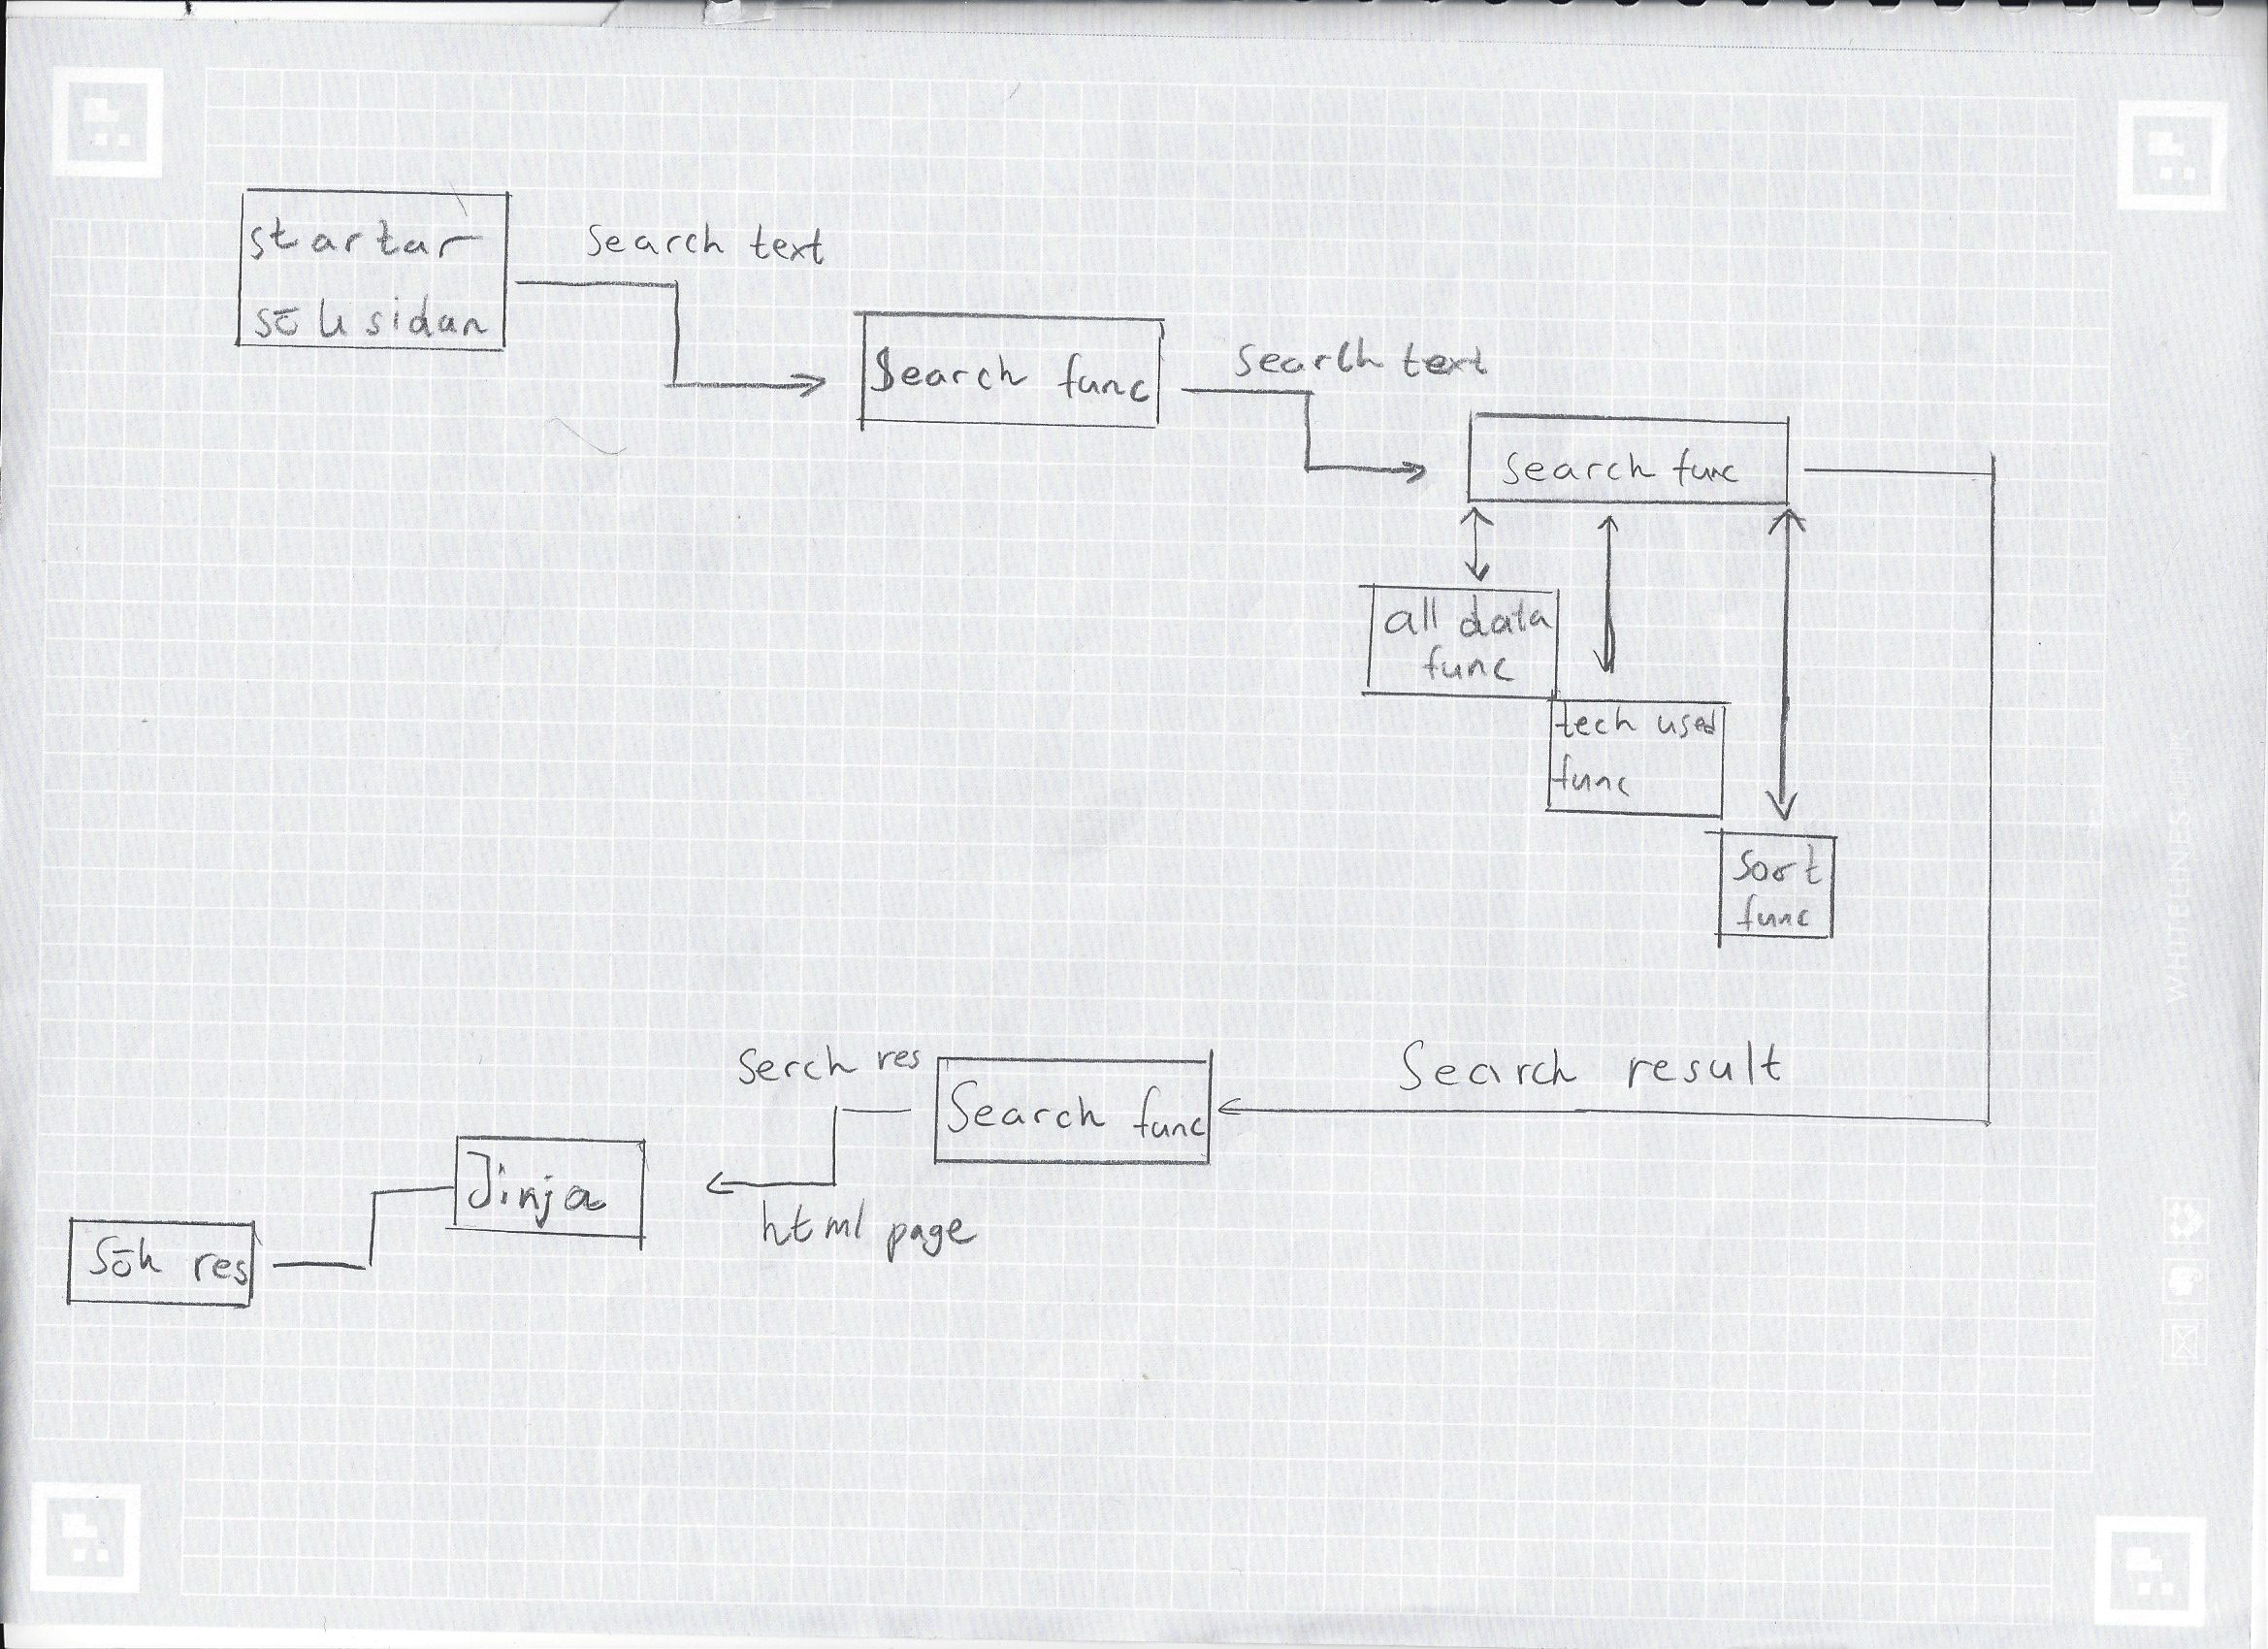
\includegraphics[width=90mm]{sekv.jpg}
\caption{Sekvensdiagram över searchfunctionen tillsammans med presentationslager}\label{sekv_dia}
\end{figure}
\pagebreak

\section{Övergripande bild}
Bilden nedan visar simpelt de tre lager vi arbetar med. Presentationslagret är delen som visar html sidor. De laddas med hjälp av jinja. Jinja blir tilldelad sidorna av Flask som ligger i ramverket. Innehållet i htmlsidorna läses från en .json fil. Den filen läses in i datalagret. Datalagret tar även hand om sökningar i data.json filen. Flask kommer kalla på specifka delar av .json filen beroende på vad användaren skickar för förfrågan. Flask returnerar sedan html sidan som ska laddas tillsammans med informationen som ska fylla sidan.

\begin{figure}[ht!]
\centering
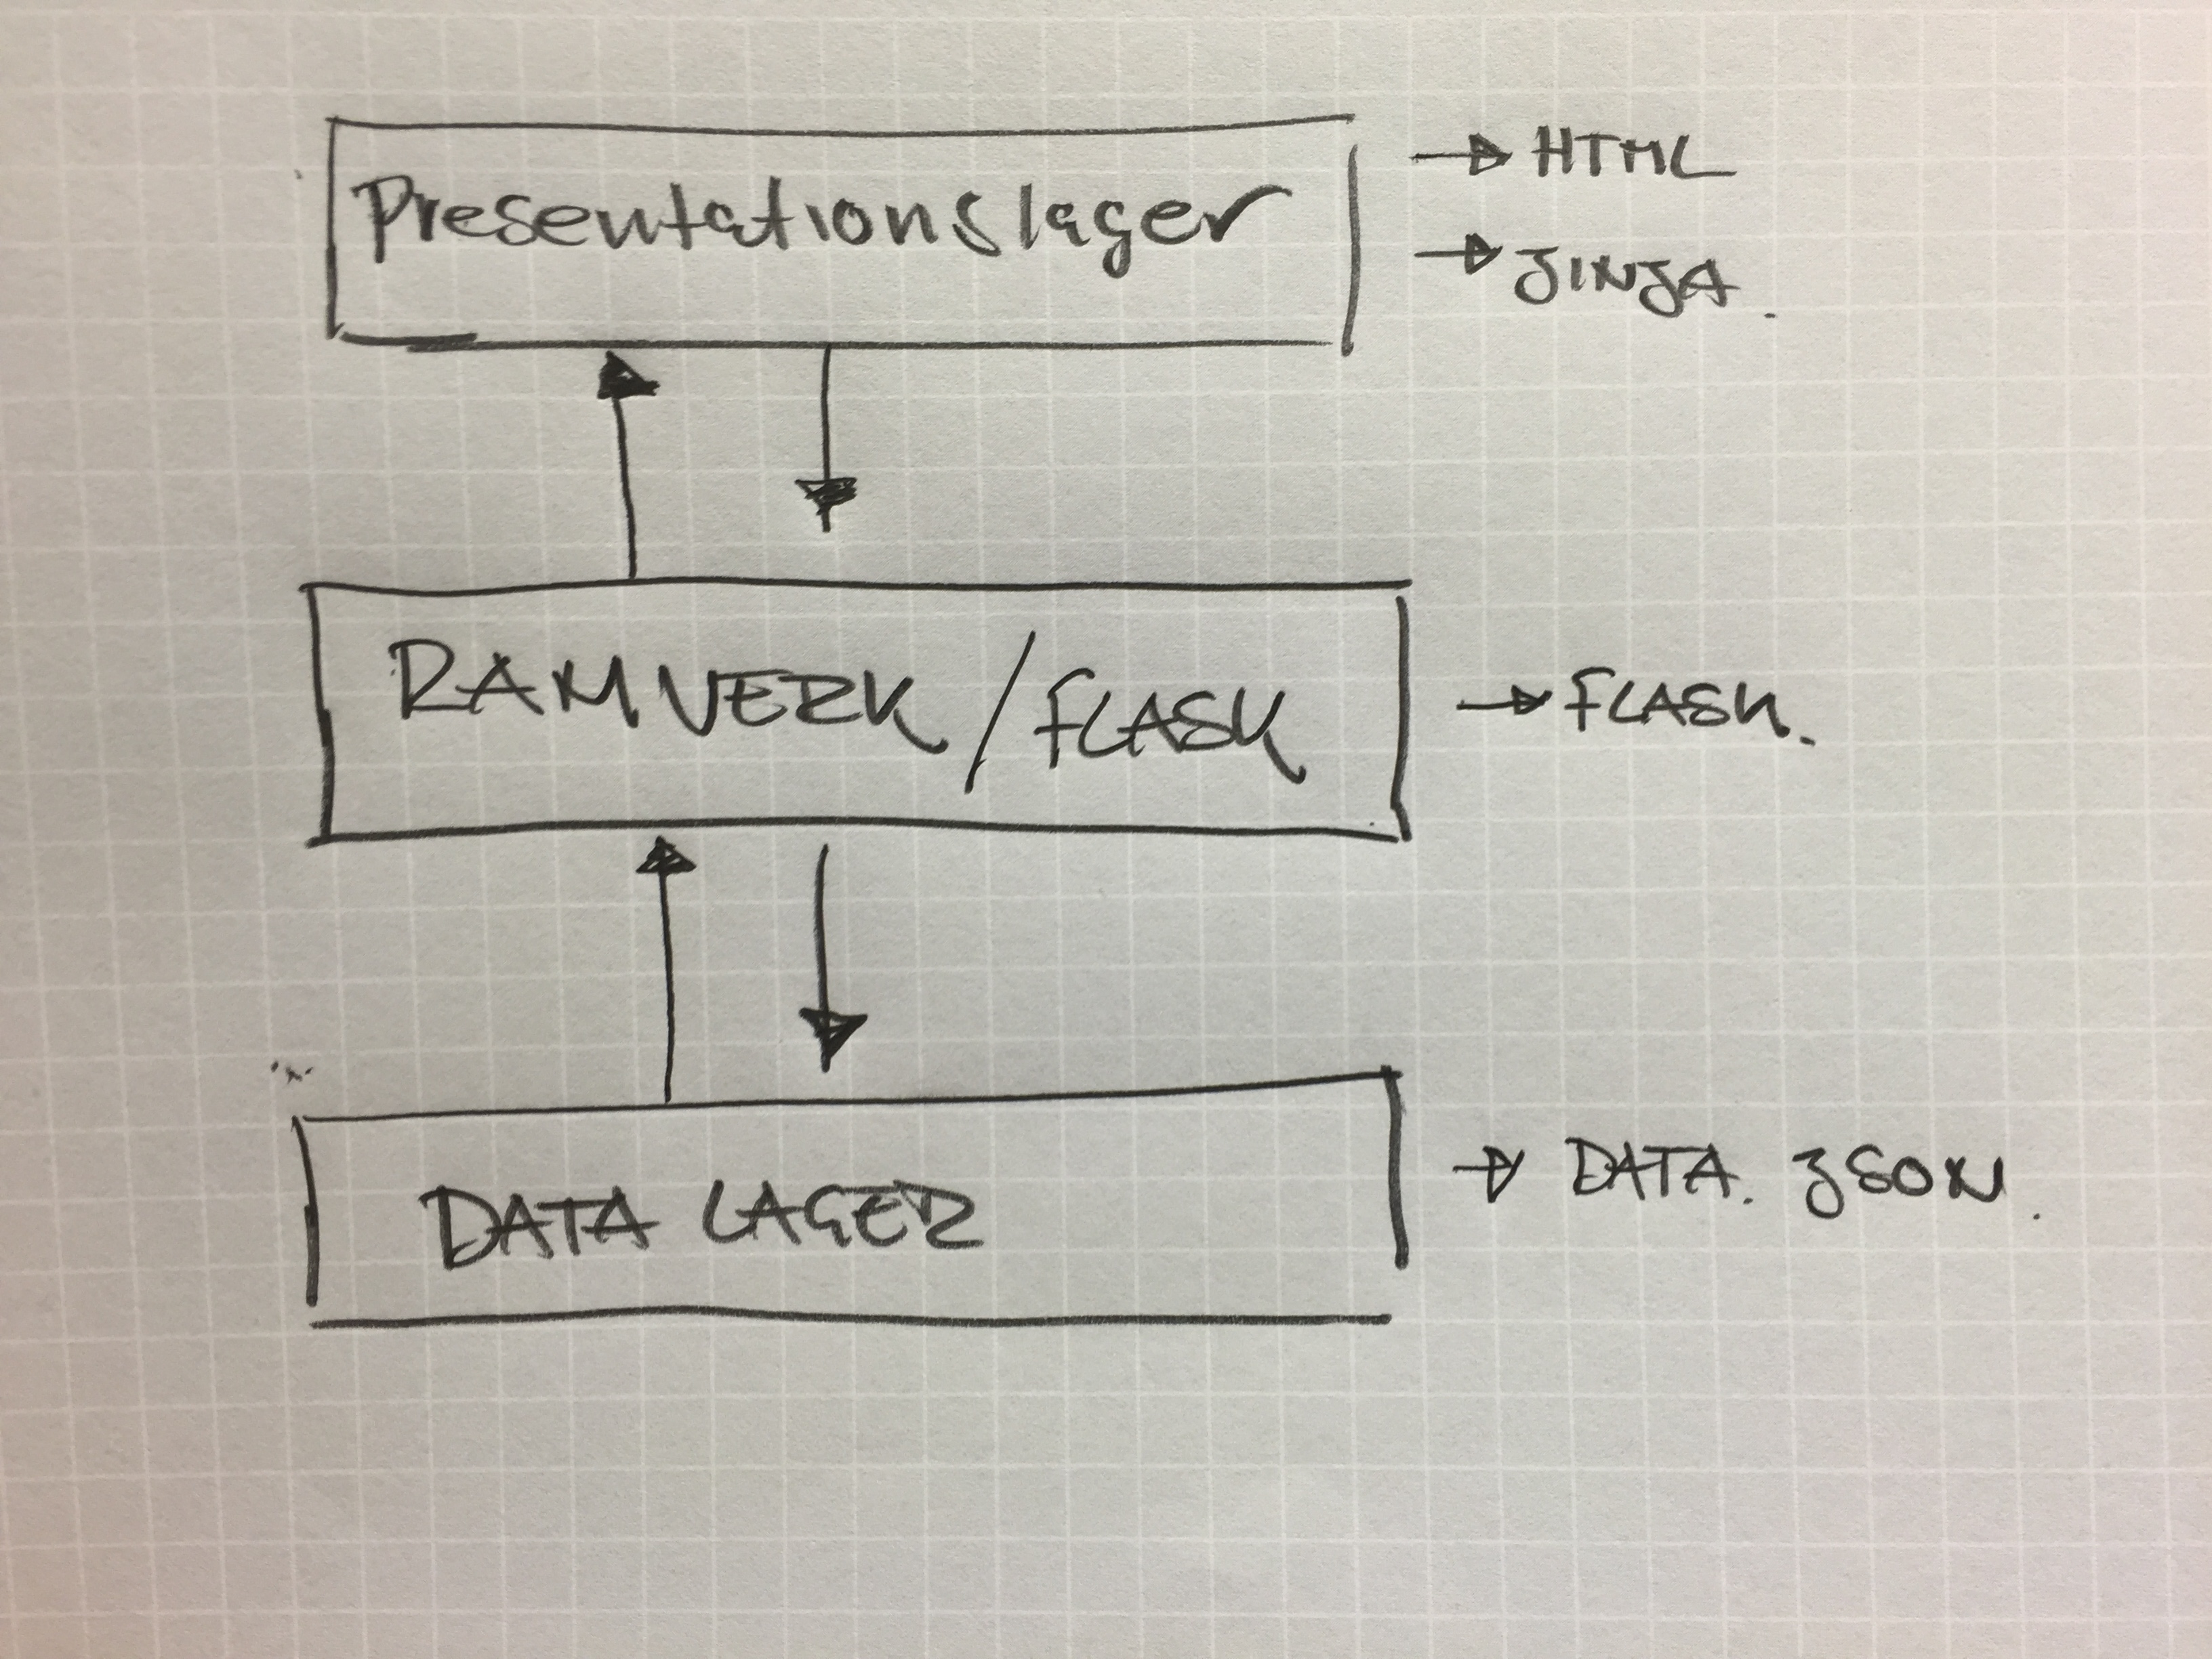
\includegraphics[width=90mm]{overgr.jpg}
\caption{Övergripande bild på hur datalager, ramverk och presentationlager kommunicerar med varandra}\label{overgr}
\end{figure}
\pagebreak

\section{Datalagret}
Här nedan kommer det finnas förklaring på funktioner som vi implemterat i vårat datalager. Här finns även sekvensdiagrammet. Det kommer till en början vara översiktligt och sedan gå mer in på djupet av varje funktion och hur de fungerar tillsammans med andra funktioner.

\subsection{Kursen datalager specifikationer}
I denna sektionen finns kursens krav på vad de olika funktionerna i datalagret ska ha. För varje funktiner kommer det finnas en koppling mellan funktionen vi skrivit och kursenskrav.

\subsubsection{Load-funktionen}
Kursenskrav: Ladda en .json fil och returnera en lista med alla projekt. Load ska ladda från en fil med UTF-8 teckenkodning. Vid error ska funktionen returnera ``None''.\\
\indent Parameterar: filnamn, en sträng som innehåller namnet på json filen vi vill ladda.\\
\indent Returnerar: en lista, listan ska inne hålle alla project från json filen eller ``None''\\
Vår funktion: \ref{over-load-func} Load-funktionen.

\subsubsection{Get-project-count-funktionen}
Kursenskrav: Få antalet project i en lista av projekt.\\
\indent Parametrar: En databaslista som man får ifrån Load-funktionen.\\
\indent Returnerar: Antalet project i listan.\\
Vår funktion: \ref{over-get-proj-cou-func} Get-project-count-funktionen.

\subsubsection{Get-project-funktionen}
Kursenskrav: Hämtar ett speciferat project från databaslistan utifrån angivet ID. Om project inte finns returneras ``None''\\
\indent Parametrar: En databaslista som man får ifrån Load-funktionen.\\
\indent \indent Projekt id:et, ett nummber som anger vilket projekt som ska hämtas\\
\indent Returnerar: En tabell med all data från ett projekt eller ``None''.\\
Vår funktion: \ref{over-get-proj-func} Get-project-funktionen.

\subsubsection{Get-techiques-funktionen}
Kursenskrav: Hämtar en lista med alla tekniker från våra projekt, de ska vara i alfabetisk ordning.\\
\indent Parametrar: En databaslista som man får ifrån Load-funktionen.\\
\indent Returnerar: En alfabetiskt sorterad lista med namnen på alla tekniker i databaslistan.\\
Vår funktion: \ref{over-get-techs-func} Get-techniques-funktionen.

\subsubsection{Get-techique-stats-funktionen}
Kursenskrav: hämta och returnerar statistik från alla tekniker speciferat i databaslistan. Nyckeln i tabellen är namnet på tekniken och nycklens värde är en lista med en tabell inuti. Den tabellen ska ha ``id'' som första nyckel med projektets ``id'' som värde. Den andra nyckeln är ``name'' den har projekets namn som värde. Id:ets och namnet värde ges av att tekniken ingår i det specifika projektet vi tittar på. I tabellen med id:et och namnen ska vara sorterade efter id:ets värde.\\
\indent Parametrar: En databaslista som man får ifrån Load-funktionen.\\
\indent Returnerar: En tabell med teknikernas statistik (se ovan).\\
Vår funktion: \ref{over-get-tech-stats-func} Get-technique-stats-funktionen.

\subsubsection{Search-funktionen}
Kursenskrav: Hämtar och sorterar projekten som matchar sökningen som angetts.\\
\indent Parametrar: 
\indent \indent En databaslista som man får ifrån Load-funktionen.\\
\indent \indent En variabel ``sort\_by'', namnet på fältet som funktionen ska sortera efter. En variabel\\
\indent \indent En variabel ``sort\_order'', anger om sorteringen ska ske fallande eller stigande.\\
\indent \indent En lista av tekniker som det returenerade projektet måste ha med. Em tom lista betyder att fältet ska ignoreras.\\ 
\indent \indent En sträng variabel ``search'', en fri text sökning.\\
\indent \indent En lista, ``search\_fields'', fältet som vi vill att fri text sökning ska ske i. Om den är tom returneras inget. Om den är ``None'' ska alla fält sökas.\\
\indent Returnerar: En lista med tabeller som innehåller alla projekt som matchade sökningen.\\
Vår funktion: \ref{over-search-func} Search-funktionen.

\subsection{Övergripande bild av Funktioner}
Den här delen beskriver översiktligt hur funktionerna fungerar även hur de hänger ihop med andra funktioner.

\subsubsection{Load-funktionen}
\label{over-load-func}
Den här funktionen laddar in all information om projekten som vi kommer ha i våran portfolio. Den hämtar projekten ur en .json fil. Den returnerar sedan en lista med varje projekt som ett element i listan. I de listan elementen ligger projektet informationen i form av en tabell. In värdet i denna funktionen är .json filens namn.

\subsubsection{Get-project-count-funktionen}
\label{over-get-proj-cou-func}
Funktionen hämtar alla projekt i våran databas och räknar antalet projekt som vi har i databasen. Den returnerar sedan antalet projekt i databasen. In värdet i denna funktion är databas filen som load-funktionen skapde.

\subsubsection{Get-project-funktionen}
\label{over-get-proj-func}
Denna funktion får ett id på projektet vi vill ha och hela databasen. Vi returnerar sedan det projektet som matchar emot id:et vi fick in. Om id:et inte finns i något projekt retuerneras ``None''. 

\subsubsection{Get-techiques-funktionen}
\label{over-get-techs-func}
Den här funktionen tar hela databasen som in värde. Den iterar sedan över hela databasen och hämtar alla tekniker som användts i alla projekt. Den returnerar sedan en sorterad lista över alla tekniker som varit med i projekten.

\subsubsection{Get-technique-stats-funktionen}
\label{over-get-tech-stats-func}
Funktionen har databasen som in värde. Den anropar sedan Get-techniques-funktionen och sparar tekinkerna. Den går sedan igenom databasen för att se om specifika projekt innehåller tekniker vi fick av Get-techniques-funktionen. Om projektet innehåller en teknik lägger vi till projektet i en lista i form av en tabell med namn och id som nycklar och projektets namn och id som värde. Vi returnerar sedan listan med tabbelerna i sig.

\subsubsection{Search-funktionen}
Search funktionen har sex stycken in värden, databasen, sort\_by (värdet vi väljer att sortera efter), sort\_order (descending eller ascedning beroende på om vi vill ha störst först eller inte när vi sorterar), techniques (om vi vill sortera efter specifika tekniker), search (ordet eller orden vi vill söka efter), search\_fields (vilka fält i databasen som vi vill söka i). Det först search funktionen gör är att anropa get-all-data-funktionen för att få vilka projekt som innehåller det vi söker efter. Vi kollar sedan om anroparen vill sortera projekten efter speciferade projekt detta gör den genom att anropa techs-used-funktionen. Sist sorterar Search-funktionen utifrån sort\_by och sort\_order detta genom att anropa sort-data-funktionen.

\subsubsection{Get-all-data-funktionen}
Invärdet i den här funktionen är databasen, search och search\_fields. Hela den här funktionens syfte är att hämta projekten som passar sökningen som användare angett. Funktionen börjar med att kolla om search och search\_fields är ``None'', är dom ``None'' returneras hela databasen. Funktionen fortsätter om förra påståendet inte stämmer. Den kollar då om search\_fields är ``None'' är den ``None'' söker vi efter search i hela databasen, funktionen returnerar projekten vi hittade med search. Vi kollar sedan om Search\_fields är tom om den är tom retuerner funktionen ``None''. Sist går funktionen genom när använderare angett både search\_fields och search. Då kollar vi i alla projekt som innehåller search\_fields och om projektet innehåller det fältet går vi in i det fältet och kollar om fältet innehåller search värdet. Stämmer det returnerar vi alla projekt som har det fältet och den sökningen.

\subsubsection{Techs-used-funktionen}
Funktionen får invärdena search (de projekten som sökningen gav oss) och techs (vilka tekniker som ska ingå i projekten). Funktionen kollar om angivna tekniker finns med i projekten som search gav oss. Den returnerar sedan projekten som innehöll de projekten som stämde överens med angivna tekniker.

\subsubsection{Sort-data-funktionen}
Den här funktionen tar in datat vi fick i search-funktionen, sort\_by och sort\_order. Funktionen sorterar sedan efter värdet angett i sort\_by. I funktionen anropas även get-sort-order, den bestämmer om det ska vara fallande eller stigande sortering.

\subsubsection{Get-sort-order-funktionen}
Invärdet är sort\_order och funktionen bestämmer om sorteringen ska ske i fallande eller stigande ordning.\pagebreak

\subsection{Detaljerad beskrivning av funktionerna}
En djupare nivå av hur funktionerna fungerar och hur de fungerar med varandra.

\subsubsection{Load-funktionen}
Vi använder angivet namn som vi fick som invärde i ett ``with'' block för att öppna filen. Eftersom filen vi läser in ifrån är en .json fil kan vi lätt läsa in filens innehåll med den inbyggda funktionen ``json.load''. Vi returnerar sedan listan med databasen. Om det av någon anledning inte gåt att läsa filen returnerar vi ``None'' som databas. 

\subsubsection{Get-project-count-funktionen}
Funktionen kollar längen av listan, altså antalet element som finns i listan. Funktionen returnerar sedan det numret vi fick fram.

\subsubsection{Get-project-funktionen}
Vi itererar igenom databasen och kollar specifikt på varje projekt. Vi jämför sedan projektets id med id:et som använder angett. Om id:et finns i något projekt returnerar vi projektet som det stämde överens med. Om angivet id inte finns i något projekt retuernerar funktionen ``None''. 

\subsubsection{Get-techniques-funktionen}
Funktionen iterar över hela inladdade databasen, den letar sedan upp fältet ``techniques-used''. För varje teknik i ``techniques-used'' lägger vi till den teknik i en lista om listan inte redan innehåller den tekniken. Vi sorterar sedan teknikerna i listan i bokstavsordning. Funktionen returnerar sedan den sorterade listan.

\subsubsection{Get-techniques-stats-funktionen}
Funktionen börjar med att anropa get-techniques och sparar undan alla använda tekniker som använts i databasen. Vi iterar sendan igenom sparade tekniker för att kolla på varje teknik en i taget. Vi skapar en dict med tekniken som nyckel. Vi iterar nu över varje projekt. Om tekniken är med i projektet lägger vi till projekts namn och id som värde för nyckeln. Innan vi börjar med nästa teknik sorterar vi värdena som tillhör varje nyckel efter id:ets stortlek. Vi börjar sedan om med nästa teknik och köra samma process. När vi gått igenom alla tekniker returnerar vi listan med tabellen.

\subsubsection{Search-funktionen}
Alla invärden i våran search funktion har fördefinerade värden ifall inget värde skulle skickas med. Deras start värde är: sort\_by=''start\_date'', sort\_order=''desc'', techniques=''None'', search=''None'', search\_fields=''None''. Search anropar sedan get-all-datafunktionen som ger tillbaka en lista. Den lista skickar search in techs-used-funktionen för att se om om sökresultaten stämmer överens med teknikerna som angetts vid anropet. Detta sker bara så länge någon teknik har angets annars hoppas detta steg över. Sista funktionaliteten som search har är att den skickar in den sökta och filtrerade databasen i sort-data-funktionen för att sortera sökesultatet enligt användarens specifikationer. Den sökta, filtrerade och sorterade listan retuneras sedan.

\subsubsection{Get-all-data-funktionen}
Vi börjar funktionen med att titta ifall search är ``None'' OCH om search\_fields är ``None''. Om detta stämmer skickar vi tillbaka hela databasen som sökresultat. Nästa koll är om search\_fields är ``None'', om detta stämmer söker vi i alla fält genom att iterera över varje projekt för sig och kolla om search får några träffar i projektet. Om search får en träff läggs det träffade projektet till i en lista. Detta sker tills det inte finns fler projekt. När alla är genomsökta skickar vi tillbaka alla projekt som fick en sökträff. Härnäst kollar vi om search\_fields är tom, om detta stämmer returnerar vi ``None'' som sökresultat. Om ingen tidigare ``if'' sats stämmer vet vi att search och search\_fields har ett värde. Så då itererar vi över insickad databas. Vi kollar sedan om sökresultat är en lista, en int eller en sträng. Om det är en sträng gör vi sökning och sökresultat till gemener. Nästa steg kolalr om fältet matchar search\_fields och att search matchar något i databasen. Om allt detta stämmer lägger vi till projektet vi hittade alla saker i en lista. När vi gått igenom alla projekt och kollat alla fält och sökvärden returnerar vi en lista av alla projekt som matchade sökningen.

\subsubsection{Techs-used-funktionen}
Vi börjar genom att itererar över sökvärdet som search-funktionen skickade in. Vi iterar sedan över alla tekniker i fall att vi vill sortera efter flera tekniker. Vi kollar sedan om teknikerna finns med med i projekten. Om teknikerna är med lägger vi till projektet i en lista. Vi returnerar sedan den listan med filtrerade projekt. 

\subsubsection{Sort-data-funktionen}
sorterar den sökda data mängden som search skickade genom att köra ``.sort'' fukntionen. Med nycklen som vi sorterar efter som värdet sort\_by hade. Vi sorterar i ordning efter reverse eller inte beroende värdet som sort-order-funktionen returnerar. Om den returnerar True sorterar vi i fallande ordning om den returnerar False sorterar vi i fallande ordning.

\subsubsection{Sort-order-funktionen}
kollar om sort\_order är ``desc''(descending) om sort\_order är ``desc'' returnerar funktionen True. Annars returnerar funktionen False. \pagebreak

\section{Ramverk / Flask}
Nedan finns funktionerna som vi skrivit i flask för att kunna ladda html sidorna med inbäddade python funktioner.

\subsection{Funktioner}
Detta är funktionerna som kallar på jinja och laddar in html sidor så de visas i vår portfolio.

\subsubsection{Data och Config - load funktionerna}
I dessa funktioner har vi hårdkodat namnet på .json filerna.
Config-load: Laddar en config fil med information som är i till exempel header och footer.\\
Data-load: Laddar databasen från en fil med information som vi sedan använder på våra hemsidor.

\subsubsection{Index-funktionen}
Denna funktion läser in senaste projektet samt hämtar information via config-load funktionen, för att generera statisk information som finns på alla sidor. Detta kan vara till exempel information av skapare, kontakt information etc.

\subsubsection{Projects-funktionen}
Html sidan som den här funktionen skapar är till för att visa alla projekt i form av en lista.
Denna funktion läser in alla projekt från databasen och skickar de vidare till presentationslagret där en html sida skapas. Mallen som används för att visa projekten är den samma som används i search-funktionen.

\subsubsection{Project-funktionen}
Html sidan som den här funktionen skapar är till för att visa ett specifikt projekt beroende på vilket id. Funktionen kommer åt id:et via urlen.
Denna funktion hämtar information om ett specefikt projekt ur databasen och skickar det till presentationslagret. 

\subsubsection{Techniques-funktionen}
Html sidan som den här funktionen skapar är till för att visa alla tekniker och projekt som använder den specifika tekniken. 
Denna funktion hämtar alla tekniker och de projekt som använder en viss teknik och skickar detta till presentationslagret. Användarna kan klicka på ett specefikt projekt och komma till project-funktionen. 

\subsubsection{Search-funktionen}
Html sidan som den här funktionen skapar är till för att visa en sökruta och klickbara check boxar. Man kan skriva en söksträng i rutan och filtrera projekt som har specifika tekniker. Sökresultat visas sedan under checkboxarna.
Denna funktion skiljer sig från de andra då den hanterar både GET och POST, i det första skedet (GET) så visas ett formulär för användaren där man kan skriva in ett sökord och klicka i tekniker. När användaren söker på ett ord så anropas funktionen med POST och då hämtas träffande projekt ur databasen. Dessa presenteras sedan för användaren med samma mall som i projects-funktionen.   

\section{Felhantering och loggning}
Fin felhantering och logging kommer finnas beskriven i den här sektionen.
\end{document}
